%% The following is a directive for TeXShop to indicate the main file
%%!TEX root = diss.tex

\chapter{One-dimensional random walks}
\label{ch:1DExample}

%=======================================
\section{Derivation of the functional equation}
\label{sec:DerFxnEqn}
%=======================================

Before we tackle the higher-dimensional random walk problems, it will be instructive to first visit the one-dimensional case, which will help illustrate the methods and ideas that we will employ throughout this work. We'll focus on one-dimensional random walk models with smalls steps (the size of each step is at most one unit in any horizontal or vertical direction). Here the step set is $\mc S \subseteq \{\um 1, 0, 1\}$, which can also be represented via the step polynomial
\begin{align}
	S = S_{\um 1}\ol{x} + S_0 + S_1 x\,.
\end{align}
\begin{figure}[H]
    \centering
    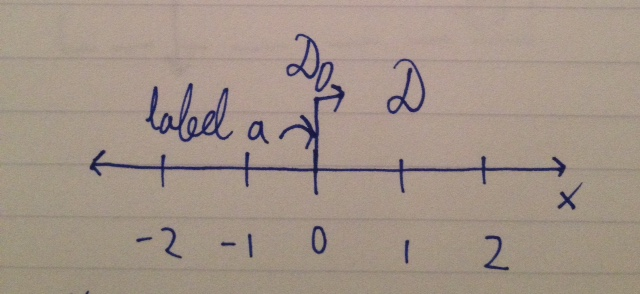
\includegraphics[scale = 0.5]{image2}
    \caption{Regions on the line}
    \label{fig:line}
\end{figure}
Here $S_k = 1$ if $k \in \mc S$ or $S_k = 0$ otherwise. Suppose that we have a walk ending on integer coordinate $n$. Then we may extend it by stepping back, staying in one place or moving forward. In the full generating function we keep track of the location of the walk with the monomial $x^n$. Then stepping back would be the same as multiplying the monomial $x^n$ by $\ol{x}$. That is, adding of coordinates corresponds to multiplication of monomials. Since each possible step is either in $\mc S$ or not, the number of possible models with small steps on the axis is $2^3 = 8$. For random walks with interactions we'll also mark every visit to the origin. For example if we have a walk ending coordinate 1 (with monomial $x$) and take a step back we multiply by $\ol x$ and obtain $x^0$. To mark this visit we also multiply by a variable $a$ that acts as a label. Thus repeated visits will result in an increase of the power of $a$.

One basic way we can build the generating function for a specific model is by a brute-force iteration. Beginning with the empty walk we will obtain all other walks by a growth process. The monomial for the empty walk is $1$ since it has length $0$ (so we have $t^0$), ends at the origin (so we have $x^0$) and has not visited the origin yet (so we have $a^0$). Then we can acquire more walks by extending the walk we have with one of the possible steps. If we have all 3 possible steps we'll have three new monomials $xt\,,t$ and $\ol xt$, since each walk is now of length 1. However, if the region is restricted, we'll have to remove some walks. Then we can repeat the procedure - extend all walks of length $n$ by one step, remove those that venture outside of the domain of interest, and mark the ones that step onto the origin. This iteration will eventually produce as many terms of the generating function as we wish by way of brute force. 

The pivotal idea is to encapsulate this process with an equation, which we can then manipulate algebraically and interpret in other ways. This idea helped produce all the generating function analysis we have in this work. Suppose that the generating function of walks of length $k$ is $Q_kt^k$. Then the full generating function is
\begin{align}
	Q = \sum_{k=0}^\infty Q_k t^k\,.
\end{align}
Using the brute-force iteration we can write a functional equation relating $Q_{k+1}$ and $Q_k$. We multiply the function $Q_kt^k$ by $tS$ to extend all the walks of length $k$ to ones with length $k+1$. Here is another key idea - we use some sort of operator $\Gamma$ that will remove all the unwanted terms and mark those at the origin, and we'll worry about its representation later. For now we have the iteration
\begin{align}
	Q_{k+1}t^{k+1} = \Gamma (tS Q_k t^k) = \Gamma(SQ_k)t^{k+1}\,.
\end{align}
In other words $Q_{k+1} = \Gamma (SQ_k)$ for all $k\ge 0$. We may sum both sides of the equation for $k\ge 0$ to reach the following equations
\begin{align}
\begin{split}
	\sum_{k=0}^\infty Q_{k+1}t^{k+1} &= \sum_{k=0}^\infty\Gamma (SQ_k)t^k\\
	Q - Q_0 &= t\Gamma  S\sum_{k=0}^\infty Q_kt^k\\
	Q &= 1 + t\Gamma (SQ)
\end{split}
\end{align}
where we factor out the $t$ since the operator only acts on monomials $x^n$ and not on $t$. We've also assumed that we could factor out $\Gamma$ from the infinite summation. We are working with formal series after all and we are looking for the easiest approach. In fact we'll use this to define how $\Gamma$ acts as an operator - it acts term-wise on the series. We may rewrite the functional equation as
\begin{align}
	\mc L Q = (1-t\Gamma S)Q = 1\,,
\end{align}
which highlights the operator nature of the equation. We can invert this operator $\mc L$ formally in the following way.
\begin{align}
	Q = \sum_{k=0}^\infty (t\Gamma S)^k(1) =   \sum_{k=0}^\infty t^k(\Gamma S)^k(1) 
\end{align}
where the operator $\Gamma S$ acts by multiplying by $S$ first and then by applying $\Gamma$ on the result. The power here indicates iteration.

All that is left to do is to find a good representation of the operator $\Gamma$. First, we need to remove all walks that end outside of the domain of interest. For illustrative purposes we'll use the domain of the nonnegative integer coordinates. We must remove any walks that venture outside of this region. However, starting with a valid walk we cannot go too far - the furthest we may go with one step is the coordinate $\um 1$ where the walk will now have monomial $a^i \ol{x} t^j$ for some $i,j\ge 0$. So, at worst, when we multiply $Q_k$ by $S$ we may pick up some terms with monomials that contain $\ol{x}$. Since we don't want these, it's enough to remove terms with monomials $\ol x$. This can easily be represented as follows. Let
\begin{align}
	E = 1 - \ext{\ol x}
\end{align}
where $1$ is the identity operator and $\ext{\ol x}$ acts on generating functions by picking out the $\ol x$ term (not just the coefficient). For the marking we can do this by picking out walks that end at 0 (counted with the term $x^0$) and multiplying them by $a$. This can be represented by the operator
\begin{align}
	L = 1 + (a-1) [x^0] = 1 + b[x^0]
\end{align}
where $b = a-1$. What this operator does is take a function and add to it $(a-1)$ times the $x^0$ term. The final function has a $x^0$ term with coefficient $1 + (a-1) = a$. We may write $\Gamma = LE$ where $L$ and $E$ act term-wise on power series in $t$ because that is the constraint we put on $\Gamma$. These operators make it easier to perform computations. For example, we may expand the product $LE$ as
\begin{align}
\begin{split}
	\Gamma &= LE = (1 - \ext{\ol{x}})(1 + b[x^0]) \\
	&= 1 + b[x^0] - \ext{\ol{x}}-\ext{\ol{x}}b[x^0]\\
	&=1 + b[x^0] -\ext{\ol{x}}\,,
\end{split}
\end{align}
which shows that the marking and removing of terms are done in parallel. The last term vanished  because once we've made the first extraction $[x^0]$ that term no longer contains a variable $x$, and the $[\ol x]$ extraction will pick out nothing. We would have found the same result if we computed $EL$ instead and this shows that the operators commute.
\begin{example} We'll now illustrate how the operators work. Suppose that $S = x + \ol{x}$. Starting with $Q_0 = 1$ we have
\begin{align}
Q_1 = LES(1) &= (1+b[x^0]-\ext{\ol{x}})(x+\ol{x}) = x+\ol{x} -\ol{x} = x\\
Q_2 = LES(Q_1) &=  (1+b[x^0]-\ext{\ol{x}})(x^2+1) = x^2 + 1 + b = a + x^2\\
Q_3 = LES(Q_2) &=  (1+b[x^0]-\ext{\ol{x}})(a\ol{x}+ax+x+x^3) \\
&= a\ol{x}+ax+x+x^3 -a\ol{x} = (1+a)x+x^3\,.
\end{align}
Therefore
\begin{align}
\begin{split}
	Q &= Q_0 + Q_1 t +Q_2 t^2+ Q_3t^3 + \cdots\\
	&= 1 + xt + (a+x^2)t^2+((1+a)x+x^3)t^3+ \cdots\,.
\end{split}
\end{align}
Note that if we apply $\Gamma$ to the resulting function $Q$ we obtain $Q$ again but with the first term $Q_0 = 1$ missing.
\end{example}
The theory so far is consistent with the present methods for finding functional equations for the generating functions for random walk models because in the end we reach the same functional equations. However, the perspective is different and this allows us to go further than before. To show the consistency with the theory so far, we'll expand the operator form and write down a functional equation that does not involve operators. For the rest of the chapter we'll use the notation $Q_k = [x^k]Q$ to reduce clutter. We start with
\begin{align}
\begin{split}
	[x^0] SQ &= [x^0]((S_{\um 1}\ol x+S_0 +S_1 x)Q) \\
	& = (S_{\um 1}\ext x +S_0\ext{\ol x} +S_1 \ext{\ol{x}^2})Q\\
	& = S_{\um 1}Q_1 + S_0 Q_0
\end{split}
\end{align}
where last line follows since $Q_{\um 1}= 0$ since that would include walks ending on $\ol x$. A similar computation shows that $\ext{\ol x}SQ = S_{\um 1} Q_0$ and this gives the functional equation
\begin{align}
\begin{split}
	1 &= Q - tLE(SQ) = Q - t(SQ + b[x^0]SQ - \ext{\ol x}SQ\\
	&= Q - t(SQ + b(S_{\um 1}Q_1 + S_0Q_0) - \ol{x}(S_{\um 1}Q_0))\,.
\end{split}
\end{align}
We can rewrite it in the following form
\begin{align}
	(1-tS)Q - t(bS_0-\ol{x}S_{\um 1})Q_0 -btS_{\um 1}Q_1 = 1\,.
\end{align}
Here $Q = Q(x)$, $Q_0 = Q(0)$ and $Q_1 = Q'(0)$. It turns out that the $Q_1$ term is not needed. To see this we first eliminate the $Q_1^1$ term by applying $[x^0]$ to both sides of the equation.
\begin{align}
\begin{split}
	 1 &= Q_1^0 - t(S_{\um 1}Q_1 +S_0 Q_0) - tbS_0Q_0 - btS_{\um 1}Q_1\\
	 &=(1-atS_0)Q_0-atS_{\um 1}Q_1\,.
\end{split}
\end{align}
We can solve this equation for $Q_1$, that is 
\begin{align}
	tS_{\um 1}Q_1 = \ol{a}((1-atS_0)Q_0-1)\,,
\end{align}
and substitute the result into the first functional equation (for now we don't worry about the possibility of $S_{\um 1} = 0$ because it leads to the same conclusion anyway). Then
\begin{align}
\begin{split}
	1 &= (1-tS)Q - t(bS_0-\ol{x}S_{\um 1})Q_0 - c((1-atS_0)Q_0-1)\\
	& = (1-tS)Q - (c -t\ol{x}S_{\um 1})Q_0 + c
\end{split}
\end{align}
and we can rewrite the equation as
\begin{align}
	(1-tS)Q - (c -t\ol{x}S_{\um 1})Q_0 = \ol{a}
\end{align}
since $1 - c = 1 - (1-\ol{a}) = \ol{a}$. We'll call this the master functional equation. 

\begin{example} When $S = x+\ol x$ we have the functional equation
\begin{align}
	(1-t(x+\ol x))Q - (c -t\ol{x})Q_0 = \ol{a}\,.
\end{align}
\end{example}
It turns out that the back substitution is unnecesary and this is a good thing because in higher dimensions we would have to perform an exponential number of back substitutions to obtain such an equation ($2^d$ where $d$ is the dimension). Previous approaches in \cite{tabbara2014exact} and \cite{wong2014confining} have only dealt with two-dimensional problems that only have a few back substitutions. It is the use of operators that allows us to circumvent the problem with back substitution. To see why consider the action of the marking operator $L$. Marking a monomial is just done by a multiplication by the indeterminate $a$. This means that to undo the marking we just need to multiply by $1/a$. That is, $L$ has an inverse and we can write it immediately.
\begin{align}
	L^{\um 1} = M = 1 + \left(\frac 1a - 1\right)[x^0] = 1- c[x^0]\,.
\end{align}
If we apply this to the functional equation, the RHS is simply $L^{\um 1} (1) = 1 - c = \ol{a}$ and the LHS is
\begin{align}
	L^{\um 1}(1-tLES)Q &= L^{\um 1}Q - tESQ \\
	&= (Q-cQ_0) - t(SQ - \ol{x}S_{\um 1}Q_0) \\
	&= (1-tS)Q - (c-t\ol{x}S_{\um 1})Q_0\,. 
\end{align}
We've arrived at the master functional equation in cleaner way.
\begin{prop} The one-dimensional random walk model restricted to the nonnegative axis, with Laurent step polynomial $S = S_{\um 1}\ol{x}+S_0 + S_1 x$, has a generating function $Q$ satisfying the functional equations
\begin{align}
	(L^{\um 1}-tES)Q &= \ol{a}\,,\\
	(1-tS)Q-(c-t\ol{x}S_{\um 1})Q_0 &= \ol{a}\,.
\end{align}
and we call them the operator and master functional equations respectively.
\end{prop}
The operator notation/perspective is powerful. It will allow us to derive functional equations for many random walk models in arbitrary dimensions with ease. Usually derivations have employed inclusion-exclusion and careful book-keeping (\cite{bousquet2010walks}, \cite{melczer2014variants}) to write master functional equations (or their precursors) in a direct manner. Unfortunately that approach is difficult to generalize to arbitrary dimensions and more dificult restrictions/marking.

We can also deal with coefficient extraction in a neater way. Instead of extracting $[x^k]$ from the master functional equation, it is better to first go through the operator equation since $[x^k]$ interacts with $L$ and $E$ in a nice way. We have
\begin{align}
	[x^0]L^{\um 1} &= [x^0]-[x^0]c[x^0] = [x^0]-c[x^0] = \ol{a}[x^0]\\
	[x^0]E &= [x^0] - [x^0]\ol{x}[\ol{x}] = [x^0]\,.
\end{align}
When we extract the $x^0$ term from the functional equation we have
\begin{align}
\begin{split}
	[x^0]\ol{a} &= \ol{a} = [x^0](L^{\um 1} - tES)Q \\
	&= ([x^0]L^{\um 1} - t[x^0]ES)Q \\
	&= (\ol{a}[x^0]-t[x^0]S)Q\\ 
	&= [x^0](\ol{a}-tS)Q\,.
\end{split}
\end{align}
Therefore we have a functional equation for the first coefficient
\begin{align}
	[x^0](1-atS)Q = 1\,.
\end{align}
We can perform the extraction immediately and it simplifies to
\begin{align}
	(1-atS_0)Q_0-atS_{\um 1}Q_1 = 1\,.
\end{align}
Extracting higher coefficients is not difficult. If $k \ge 1$ we have
\begin{align}
	[x^k]L^{\um 1} &= [x^k]-[x^k]c[x^0] = [x^k]\,,\\
	[x^k]E &= [x^k] - [x^k]\ol{x}[\ol{x}] = [x^k]\,,
\end{align}
and
\begin{align}
\begin{split}
	[x^k]\ol{a} = 0 &= [x^k](L^{\um 1} - tES)Q \\
	&= ([x^k] - t[x^k]S)Q \\
	&= [x^k](1-tS)Q\,.
\end{split}
\end{align}
This extraction translates to the equation
\begin{align}\begin{split}
	Q_k - t(S_{\um 1}Q_{k+1}+S_0Q_k+S_1 Q_{k-1}) &= 0\\
	 (1-S_0t) Q_k -t(S_{\um 1}Q_{k+1} + S_1 Q_{k-1}) &= 0\,.
\end{split}\end{align}

\begin{prop} The one-dimensional model with  $S = S_{\um 1}\ol{x}+S_0 + S_1 x$ has generating functions $[x^k]Q = Q_k$ for the walks ending at coordinate $k$ satisfying the following functional equations
\begin{align}
	(1-atS_0)Q_0-atS_{\um 1}Q_1 = 1\,,\\
	 (1-S_0t) Q_k -t(S_{\um 1}Q_{k+1} + S_1 Q_{k-1}) &= 0\,,
\end{align}
where $k\ge 1$ in the second equation.
\end{prop}

%=======================================
\section{Solving the functional equation for various $S$}
\label{sec:Solving1D}
%=======================================
The one-dimensional random walk models have algebraic generating functions while the higher-dimensional generalizations may not even have D-finite generating function (in the variable $t$). Nevertheless the one-dimensional models allow us to showcase some of the methods we'll use later on in the higher-dimensional settings. This is just an observation, but the difficulties in retrieving the solutions tend to scale up when we have more steps with negative coordinates. Those are steps that allow random walks to go back closer to the axes and origin. Although it may be surprising, this is a consequence of the form of the master functional equation - the coefficients become more complicated. We begin with the easier case.
%=======================================
\subsection{The $S_{-1} = 0$ case.}
%=======================================
This condition allows us to find $Q_0$ directly from the $[x^0]$ equation.
\begin{align}
	Q_0 = \frac{1}{1-aS_0t}\,.
\end{align}
We can substitute this into the master functional equation.
\begin{prop} The generating function $Q$ for random walk models with small steps on the half-line with $S_{\um 1} = 0$ is given by
\begin{align}
	Q(x,a;t) =\frac{\ol{a}}{1-tS}\left(1 + \frac{b}{{1-atS_0}}\right) = \frac{1-tS_0}{(1-tS)(1-atS_0)}\,.
\end{align}
\end{prop}
This takes care of the less interesting half of all 8 models. Note the relationship between $Q(x,a;t)$ and $Q(x,1;t)$, where the latter function is the generating function for the unmarked problem. When we set $a = 1$ in the above equation we find
\begin{align}
	[b^0]Q = \wh{Q} =  \frac{1-S_0t}{(1-st)(1-S_0t)}\,.
\end{align}
By inspection we can see that
\begin{align}
	(1-aS_0t)Q-(1-S_0t)\wh{Q} = 0\,,
\end{align}
which we may write as $B((1-aS_0t)Q)  = 0$ using the operator $B = 1- [b^0]$. There's a similar relationship for $Q_0$. Extracting $[x^0]$ from the last equation leads to
\begin{align}
	B((1-aS_0t)Q_0) = 0
\end{align}
and thus we have
\begin{align}
	Q_0 = \frac{1-aS_0t}{1-S_0t}\wh{Q}_0\,.
\end{align}
\begin{prop} Let $B = 1 - [b^0]$ and let $Q$ be the generating function for a random walk model with small steps on the half-line with $S_{\um 1} = 0$. Then $Q$ satisfies the functional equations
\begin{align}
	B((1-aS_0t)Q) = 0\com B((1-aS_0t)Q_0) = 0\,.
\end{align}
In other words
\begin{align}
	Q = \frac{1-aS_0t}{1-S_0t}\wh{Q}\com Q_0 = \frac{1-aS_0t}{1-S_0t}\wh{Q_0}\,.
\end{align}
\end{prop}
Even such small examples already show connections between $Q$ and $\wh Q$. It will be interesting to find such relationship for higher-dimensional random walk models.
%=======================================
\subsection{The $S_{-1} \neq 0$ case.}
%=======================================
In this case we will apply the Obstinate Kernel as is done in the two-dimensional cases in \cite{tabbara2014exact}, page 11 of \cite{wong2014confining}. ZZCITEZZ It requires finding an $x$ value that makes the kernel $K = 1 - tS$ vanish in the functional equation
\begin{align}
	(1-tS)Q - (c -t\ol{x})Q_0 = \ol{a}\,.
\end{align}
Such a solution will exist since $S_{\um 1} = 1$ and therefore the equation $1 - tS = 0$ is nontrivial and has degree in $x$ at least 1. Let one such solution be $x = \sigma$ and suppose that we can substitute it into the functional equation. ZZCITEZZ For now we have to assume that the whole term $KQ$ vanishes and we obtain
\begin{align}
	- (c - t\ol{\sigma})Q_0 = \ol{a}\,.
\end{align}
Then
\begin{align}
	Q_0 = \frac{\ol{a}}{\ol{\sigma}t-c}
\end{align}
and now we can solve for $Q$ explicitly
\begin{align}
	Q = \frac{\ol{a}}{1-tS}\left(1 - \frac{t\ol{x}-c}{t\ol{\sigma}-c}\right) = \frac{t}{1-tS}\left(\frac{\ol{x}-\ol{\sigma}}{b-a\ol{\sigma}t}\right) = \frac{t(\sigma-x)}{x(1-tS)(b\sigma-at)}\,.
\end{align}
\begin{prop} For a random walk model with small steps on the half-line with $S_{\um 1} = 1$, let $\sigma$ be a root of $K$ that makes $KQ$ vanish. Then generating function $Q$ is given by
\begin{align}
	Q &= \frac{t}{1-tS}\left(\frac{\ol{x}-\ol{\sigma}}{b-a\ol{\sigma}t}\right)
\end{align}
and it has a first term
\begin{align}
	Q_0 = \frac{\ol{a}}{\ol{\sigma}t-c}\,.
\end{align}
Here $\sigma$ depends on the rest of the step set $\mc S$.
\end{prop}
As before we can find a linear relationship between $Q(x,a;t)$ and $Q(x,1;t)$.
\begin{prop} Let $B = 1 - [b^0]$ and let $Q$ be the generating function for a random walk model with small steps on the half-line with $S_{\um 1} = 1$. Then $Q$ satisfies the functional equations
\begin{align}
	B((a\ol{\sigma}t-b)Q) = 0\com B((a\ol{\sigma}t-b)Q_0) = 0\,.
\end{align}
In other words
\begin{align}
	Q = \frac{t}{at-b\sigma}\wh Q \com Q_0 = \frac{t}{at-b\sigma}\wh{Q_0}\,.
\end{align}
\end{prop}

The final task for this section will be to find what $\sigma$ will be for various cases. We already know $S_{\um 1} \neq 0$ so the result depends on $S_0$ and $S_1$. In general the kernel is zero when
\begin{align}\begin{split}
	t S &= 1\\
	t(S_{\um 1} + S_0 x + S_1 x^2) &= x\\
	tS_1 x^2 -(1-S_0t)x + tS_{\um 1} &= 0\,.
\end{split}\end{align}

When $S_1 = 0$ we have the equation $(1-S_0t)x = t$ so the single root is
\begin{align}
	\sigma = \frac{t}{1-S_0t}\,.
\end{align}

When $S_1 = 1$ the equation $tx^2 -(1-S_0t)x + t = 0$ is quadratic with two roots that are functions of $t$. We have to pick the one which has no singularity at $t = 0$. The roots are
\begin{align}
\sigma = \frac{1-S_0t - \sqrt{(1-S_0t)^2-4t^2}}{2t}, \quad \sigma^\ast = \frac{1-S_0t + \sqrt{(1-S_0t)^2-4t^2}}{2t}\,,
\end{align}
and they multiply to 1 so $\ol{\sigma} = \sigma^\ast$. Note that in the relationship between the marked and unmarked $Q_0$ we have
\begin{align}
	Q_0 = \frac{t}{at-b\sigma}\wh{Q_0}
\end{align}
where $\sigma$ is a function containing a square root, i.e. not a polynomial. However we can look at the problem from a different angle - that of the Algebraic Kernel method used extensively in the quarter-plane model classification ZZCITEZZ. We find a polynomial $f(a,t)$ for which $B(fQ_0) = c$. This will serve to illustrate the group approach together with the kernel method. Both of the cases we need to consider have $S_{\um 1} = S_1 = 1$ with $S_0$ equal to 0 or 1. This means that $S$ is invariant under the map $\ast: x \mapsto \ol{x}$. This map allows us to write another functional equation and we have the system
\begin{align}
	(1-tS)Q - (c -t\ol{x})Q_0 - \ol{a}=0\,,\\
	(1-tS)Q^\ast - (c -tx)Q_0 -\ol{a}=0\,.
\end{align}
To eliminate the $Q_0$ term we multiply the first equation by $c -tx$, the second by $c -t\ol{x}$ and subtract one equation from the other. We divide everything by $1-tS$ and the equation that remains is
\begin{align}
	(c-tx)Q(x) - (c-t\ol{x})Q(\ol{x}) -\ol{a}\delta &= 0\,,
\end{align}
where
\begin{align}
	\delta =\frac{t(\ol{x}-x)}{1-tS}
\end{align}
and crucially $\delta$ doesn't depent on $a$. We extract the $x^1$ coefficient from the equation to acquire an equation relating $Q_1$ and $Q_0$
\begin{align}
	c Q_1 - t Q_0 - \ol{a}\delta_1 = 0\,.
\end{align}
We can set $a = 1$ here to find that
\begin{align}
	-\delta_1 = t \wh{Q_0}
\end{align}
which we can substitute back into the original equation as follows.
\begin{align}
\begin{split}
	c Q_1 &= t Q_0 - \ol{a} t \wh{Q_0}\\
	b Q_1 &= t (aQ_0 - \wh{Q_0})\,.
\end{split}
\end{align}
Earlier we had the equation
\begin{align}
	(1-aS_0t)Q_0 = 1 + a S_{\um 1} t Q_1 = 1 + at Q_1
\end{align}
which we can solve for $Q_1$ this time and insert the solution into the above equation
\begin{align}
	b ((1-aS_0t)Q_0-1) = t^2 a (aQ_0 - \wh{Q_0})\,.
\end{align}
Collecting coefficients and simplifying leads us to the equations
\begin{align}
\begin{split}
	(b(1-aS_0t)-a^2 t^2) Q_0 -(-at^2)\wh{Q_0} =& b\,,\\
	(c(1-aS_0t)-a t^2) Q_0 -(-t^2)\wh{Q_0} =& c\,.
\end{split}
\end{align}
This gives $f(a,t) = c(1-aS_0t)-a t^2$.
\begin{prop} When $S_{\um 1} = S_1 = 1$ we have
\begin{align}
	B((c(1-aS_0t)-a t^2)Q_0) = c.
\end{align}
\end{prop}
With two different approaches we obtained slightly different relationships upon applying the operator $B$.
%=======================================
\subsection{Conclusion}
%=======================================
In this section we were able to find explicit solutions for $Q_0, Q$ and also $B$-operator relationships for $Q$ and $\wh Q$. In higher dimensions this analysis will be more difficult, but we will find some $B$-operator relationships for the functions equivalent to $Q_0$ and $\wh{Q_0}$. Here is a table showing the resuls for the one-dimensional random walk models with small steps and interaction with the origin. Here $\sigma$ depends on $S_1$ and $S_0$.
 \begin{table}[H]
    \caption{Generating functions for walks with small steps on the nonnegative half-line.}
    \label{tbl:table1d}
    \centering
    \begin{tabular}{ccccc}
    \toprule
    Case & $S$ & $Q_0$ & $Q$ & $f(a,t)$\\
    \midrule
    $S_{\um 1} = 0$ & $S_0 + S_1 x$ & $\dfrac{1}{1- a S_0t}$ & $\dfrac{1-S_0 t}{(1-tS)(1-atS_0)}$ & $1-atS_0 $ \\
    $S_{\um 1} = 1$ & $1+S_0+S_1 x$ & $\dfrac{\sigma}{at - b\sigma}$ & $\dfrac{t(x- \sigma)}{x(1-tS)(at-b\sigma)}$ & $a\ol \sigma t-b$\\
    Add the two subcases &&&&\\
    \bottomrule
    \end{tabular}
\end{table}

\endinput
